\chapter{A semiclassical approach to SHE}

\label{chapter3}

In this chapter, we shall look at the semi-classical picture of SHE and try to understand the mechanisms behind the phenomena.

\section{SHE revisited: relation with AHE}

As seen in \cref{sec:ohe}, the OHE results in a charge imbalance along the edges of the conductor in the presence of an external magnetic field. We have also seen that in the case of SHE (sec \ref{sec:she}), instead of a charge imbalance, we see a spin imbalance i.e. a preferential accumulation along the edges of the material.

Both AHE and SHE are similar in the way that there is a spin imbalance and hence an accumulation of carriers with opposite spins on opposite edges of the sample.
The only difference is that in the case of AHE, there is a net magnetization of the material (since we typically use magnetic materials for AHE).
This gives preferential scattering of the carriers based on spin but with unequal proportion i.e. due to the net magnetization of the material, the proportion of spin up \( \uparrow \) and spin down \( \downarrow \) is unequal and hence there will be disproportionate accumulation of one spin ($ \uparrow $ or $ \downarrow $) from another ($ \downarrow $ or $ \uparrow $).

A significant advantage of SHE over AHE is that the former doesn't require an external magnetic field to function.
As long as the material in question possesses a high spin-orbit interaction, SHE is observed and the conversion of pure charge current (unpolarized electrons) gets converted into pure spin current (polarized electrons) with no charge current \cite{hirsch1999spin}.

\subsection{Spin Hall Angle (SHA)}

\label{subsec:spin-angle}

A parameter of importance in the context of SHE, is the spin Hall angle \( \theta_{SH} \) which is defined as

\begin{equation} \label{eq:sha}
    \theta_{SH} = \frac{\sigma^s_{xy} \: e}{\sigma^c_{xx} \: \hbar}
\end{equation}

where \( \sigma^s_{xy} \) is the transverse conductivity due to spin current, \( \sigma^c_{xx} \) is the longitudinal conductivity due to charge current, and \( e \) is the charge of an electron.

\( \theta_{SH} \) is the ratio of spin Hall conductivity to charge conductivity and quantifies the efficiency of conversion from charge to spin current and vice-versa.

\subsection{An overview of spin orbit interaction}

\begin{figure}[h!]
    \centering
    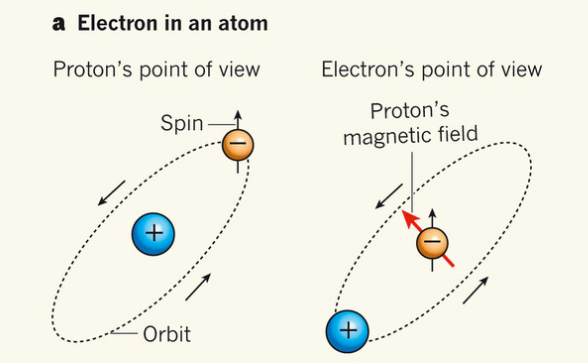
\includegraphics[scale=0.4]{soc.png}
    \caption{Relative motion of nucleus around the electron.\\ \vspace{0.2cm} \textit{Image courtesy: Binghai Yan, ``Spin-orbit coupling: A relativistic effect", Summer school on ``Topological Matter States 2016''}}
    \label{fig:soc-atom}
\end{figure}

Consider a hydrogen atom where we take the electron's frame of reference as depicted in \cref{fig:soc-atom}.
In this frame, the positively charged nucleus (a single proton in this case) revolves around the electron.
This induces a magnetic field\footnote{\Cref{eq:B-field-ring} is easily derivable using Biot-Savart or Ampere's law.} due to the moving proton, along the direction which is perpendicular to the plane of trajectory of the proton and whose magnitude is given by

\begin{equation} \label{eq:B-field-ring}
    B = \frac{\mu_0 I}{2r}
\end{equation}

Each electron has an associated intrinsic spin, which induces a corresponding spin angular momentum.
This spin also induces a spin magnetic dipole moment \( \vec{\mu}_s \), which is given by:

\begin{equation} \label{eq:mu_sS}
    \vec{\mu}_s = g_s \frac{e}{2m} \cdot \vec{S}
\end{equation}

where \( g_s \) is the gyromagnetic ratio (\( \approx 2 \) for an electron) and \( \vec{S} \) is the spin angular momentum of the electron.

This presents the scenario where the magnetic dipole is in presence of an external magnetic field (due to the moving proton) and hence will feel a torque \( \vec{\tau} \) which tries to align \( \vec{\mu}_s \) in the direction of \( \vec{B} \) and is given by

\begin{equation}
    \vec{\tau} = \vec{\mu}_s \times \vec{B}
\end{equation}

This torque \( \vec{\tau} \) will change the energy of the electron by an amount:

\begin{equation} \label{eq:dipole-energy}
    \Delta U = - \vec{\mu}_s \cdot \vec{B}
\end{equation}


\subsubsection{Spin Orbit Coupling (SOC)}

Spin orbit coupling refers to the interaction between the spin angular momentum of electron and the orbital angular momentum of the atom.

Referring to \cref{fig:soc-atom}, the orbital angular momentum \( \vec{L} = m \vec{r} \times \vec{v} \) of the atom is related to the magnetic field \( \vec{B} \) by

\begin{equation} \label{eq:BL}
    \vec{B} = \frac{\mu_0 Z e \vec{L}}{4 \pi m_e r^3}
\end{equation}

We see from \cref{eq:BL} and \cref{eq:mu_sS} that

\begin{equation*}
    \vec{\mu}_s \propto \vec{S} \quad \text{and} \quad \vec{B} \propto \vec{L}
\end{equation*}

Applying the above relations in \cref{eq:dipole-energy}, we get

\begin{equation}
    \Delta U \propto \vec{S} \cdot \vec{L}
\end{equation}

This means that orbital angular momentum of the nucleus and the spin angular momentum of the electron interact with each other, which results in the energy of the energy levels of the electrons in the atom.
This is called the \underline{spin-orbit interaction}.

\section{Mechanisms behind the phenomena}

\label{sec:mechanisms}

Over the past century, the scientific community has agreed upon three plausible mechanisms responsible for SHE. These are categorized into extrinsic and intrinsic mechanisms. Let's dive into the details of the same.

\subsection{Extrinsic}

\begin{figure}[h!]
    \centering
    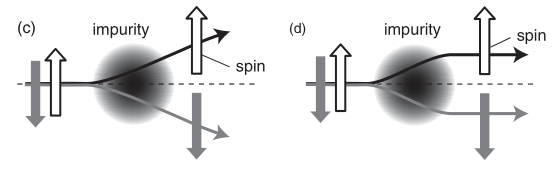
\includegraphics[scale=0.6]{she-mechanisms.png}
    \caption{Extrinsic scattering mechanisms responsible for SHE: (c) skew-scattering and (d) side jump\\ \vspace{0.2cm} \textit{Image courtesy: \cite{murakami2015spin}}}
    \label{fig:skew-vs-side}
\end{figure}

We know that for a material to exhibit SHE, spin-orbit interaction is required. One such origin of SOC is due to impurities in the sample, giving to rise "extrinsic" mechanisms of the forms:

\begin{enumerate}
    \item Asymmetric scattering (skew-scattering)
    \item Side-jump mechanism
\end{enumerate}


\subsection*{Skew-scattering}

Particles with intrinsic spin in the presence of SOC, are preferentially scattered by a central potential \cite{mott1964w}.
This central potential is due to the impurities in the sample.

Let us consider a case in two dimensions i.e. \( x-y \) plane and that the impurities are spherically symmetric.
In the presence of SOC, the impurities conserve orbital angular momentum \( L_z \) and spin angular momentum \( S_z \) separately.
As the particles cross the vicinity of such impurities, the corresponding scattering cross-section depends on the relative sign of \( L_z \) and \( S_z \) along with the angle of scattering.
For example, a greater ratio of spin \( \uparrow \) electrons will be scattered towards states of positive \( L_z \) (say) than towards states of negative \( L_z \).
This would result in more spin \( \uparrow \) electrons getting scattered to the left than to the right.
A similar analogy but opposite in direction, is applicable for spin \( \downarrow \) electrons.
The direction of scattering also depends on the nature of interaction of the impurities i.e. if interaction between the impurity and electron is attractive or repulsive in nature.

\begin{figure}[h!]
    \centering
    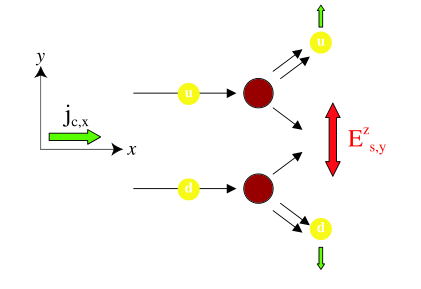
\includegraphics[scale=0.6]{skew-scattering-cls.png}
    \caption{Semiclassical picture of skew-scattering mechanism\\ \vspace{0.2cm} \emph{Image courtesy: G. Vignale. "Ten Years of Spin Hall Effect".} }
    \label{fig:semiskew}
\end{figure}

We proceed to calculate the contribution of skew-scattering towards SHE as described in \cite{Vignale_2009}.

Let us introduce a Fermi distribution along the direction of charge current \( j_{c,x} \) where superscripts \( c \) and \( x \) denote pure charge current and direction of propagation respectively.
An interesting analogy would be to consider an equivalent "spin electric field" \( E_{s,y} \) (refer \cref{fig:semiskew}) in the transverse direction which essentially pushes electrons in the \( y \) direction, with corresponding resistivity given as

\begin{equation*}
    \rho_{ss} = \frac{m^*}{ne^2 \tau_{ss}}
\end{equation*}

where \( n \) is the electron number density, and \( \tau_{ss}^{-1} \) is the skew scattering rate.
This gives us the relation between the "spin electric field" and longitudinal charge current density as

\begin{equation} \label{eq:spin-rho}
    E_{s,y} = \rho_{ss} \: j_{c,x}
\end{equation}

The spin electric field is responsible for spin current along the transverse direction, which is related by the linear relation,

\begin{equation} \label{eq:spin-drude}
    j_{s,y} = \sigma_s E_{s,y}
\end{equation}

where \( \sigma_s \) is the spin conductivity and \( j_{s,y} \) is the corresponding spin current density in the \( y \) direction.

Using simple Drude model, we also relate the longitudinal charge current density \( j_{c,x} \) and longitudinal conductivity \( \sigma_c \) by the relation

\begin{equation} \label{eq:drude}
    j_{c,x} = \sigma_c E_x
\end{equation}

where \( E_x \) is the corresponding electric field along \( x \) direction.

Multiplying equations \ref{eq:spin-rho}, \ref{eq:spin-drude} and \ref{eq:drude}, and further cancelling common terms, we get contribution to SHE via skew-scattering as

\begin{equation} \label{eq:skew-conductivity}
    \boxed{\frac{j_{s,y}}{E_x} = \sigma_{ss}^{SHE} \equiv \sigma_s \rho_{ss} \sigma_c}
\end{equation}


\subsection*{Side-jump}

Similar to skew-scattering, this mechanism is extrinsic in nature and depends on the spin-orbit interaction with the impurities.

However in contrast to skew-scattering, as seen from the schematic diagram in \cref{fig:skew-vs-side}, in this mechanism, there is a shift in the transverse component of velocity of the electrons, which arises from considering the electron as a wave packet (see \cref{fig:side}) with the collision, leading to an instantaneous change in the average momentum of the wave packet \cite{berger1970side}.

\begin{figure}[h!]
    \centering
    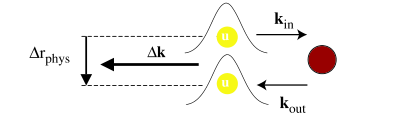
\includegraphics[scale=0.6]{packet.png}
    \caption{A semiclassical diagram of side-jump mechanism during a head-on collision with an impurity.\\ \vspace{0.2cm} \emph{Image courtesy: G. Vignale. "Ten Years of Spin Hall Effect".}}
    \label{fig:side}
\end{figure}

We shall not dive into the mathematical details of the mechanism for the sake of brevity.


\subsection{Intrinsic}

As opposed to the extrinsic mechanisms described in earlier sections, the intrinsic mechanisms cause spin-dependent transverse scattering to occur due to the spin orbit interaction with the electronic band structure of the material.

In the case of extrinsic mechanisms, a gain in transverse velocity is observed \emph{during} the scattering events.
Meanwhile, in the case of intrinsic mechanisms, the transverse velocity gain is seen \emph{between} the scattering events \cite{hoffmann2013spin}.

We shall not go over the mathematical intricacies of the mechanism for the sake of brevity.
